\subsubsection{Quarkonia Suppression and Enhancement}
\label{Sec:Quarkonia}


Theoretical studies of heavy quarkonia in QCD matter are carried out both from first 
principles using lattice-discretized QCD computations~\cite{Bazavov:2009us,Kaczmarek:2012ne} 
and within  effective model approaches. The latter aid in interpreting the lattice results and 
form the bridge to phenomenological implementations in heavy-ion collisions.

One of the key quantities computed in lattice QCD is the free energy, $F_{Q\bar Q}(r,T)$, 
of a static $Q\bar Q$ pair at distance $r$ in a medium at temperature $T$. In the vacuum it reduces to the well-known Cornell 
potential between the two quarks, but in the medium an additional entropy term develops, 
$F_{Q\bar Q}= U_{Q\bar Q} - T S_{Q\bar Q}$. Accurate calculations for $F_{Q\bar Q}(r,T)$, which are 
now available for full QCD with realistic light quark masses, show marked deviations from 
its vacuum form, through a progressive ``Debye screening" toward smaller distances 
as temperature increases. When utilizing the free energy as a potential in a Schr\"odinger 
equation~\cite{Digal:2001iu}, the charmonium groundstate, \Jpsi\, dissolves slightly above 
the critical temperature, while the excited states melt at or even below $T_{c}$; only the 
bottomonium groundstate, $\Upsilon$, survives up to 2-3\,$T_c$. On the other hand, if the 
potential is approximated with the internal energy, $U_{Q\bar Q}$, the \Jpsi\ survives to 
significantly higher temperatures, possibly up to 2\,$T_c$. These limiting cases are sometimes 
referred to as weak- and strong-binding scenarios, respectively. It has also become clear 
that a proper inclusion of absorptive processes in the $Q\bar Q$ system, characterizing its 
dissociation by dynamical processes, is essential to arrive at a realistic and quantitative description 
of its in-medium properties. 

Lattice computations also provide detailed information on $Q\bar Q$ correlation functions 
in euclidean space-time (where the ``imaginary-time" coordinate is related to the temperature 
of the system). Extracting the physical (real-time) $Q\bar Q$ spectral function requires an 
inverse integral transform on a limited number of ``data" points. This usually is done using 
maximum likelihood methods~\cite{Asakawa:2000tr,Aarts:2007pk}, sometimes guided by a 
parametric ansatz for the spectral function~\cite{Ding:2012sp}. In the bottomonium sector one 
can additionally utilize nonrelativistic heavy-quark effective theory~\cite{Aarts:2014cda}. 
The heavy-quark transport coefficient has been extracted from the low energy limit of the 
spectral functions in quenched QCD (no dynamical 
quarks)~\cite{Banerjee:2011ra,Ding:2012sp,Kaczmarek:2014jga}, highlighting the close connection 
between quarkonia and open heavy flavor in the QGP (cf.~Section~\ref{Sec:OpenHF}). The 
``reconstructed" charmonium spectral functions from lattice QCD have not yet led to definite
conclusions about the fate of bound states in the QGP. A promising complementary source of 
information are spatial correlation functions~\cite{Karsch:2012na,Bazavov:2014cta}; they are 
related to the 3-momentum dependence of the quarkonium spectral functions, but also encode 
information on modifications of the spectral (energy) strength in medium.   

Fruitful connections to lattice QCD results have been established with potential models, 
either through a Schr\"odinger equation~\cite{Mocsy:2005qW} or a thermodynamic $T$-matrix 
formulation~\cite{Cabrera:2006wh}. Here, the calculated  spectral functions can be 
straightforwardly integrated to obtain the euclidean correlation functions computed on the 
lattice. Both strong- and weak-binding scenarios for the $Q\bar Q$ appear to be compatible 
with the lattice data, once absorptive parts and a proper treatment of the continuum are 
included in the calculations. A better discrimination power arises when analyzing the 
interactions of open heavy flavor with the medium. This has been pursued in the $T$-matrix 
approach~\cite{Riek:2010fk}; only the strong-binding scenario produces sufficient strength 
in the heavy-quark transport coefficient to come close to open heavy-flavor observables in 
heavy-ion collisions (cf.~Section~\ref{Sec:OpenHF}).      
Recent progress in the determination of the in-medium $Q\bar Q$ potential has been made by 
utilizing the spectral functions of the so-called Wilson loop correlator, including absorptive
parts~\cite{Burnier:2014ssa}. Here, the real part of the potential turns out to be close to 
the free energy. Further theoretical work, exploiting the insights derived from both lattice QCD and 
effective models, is needed to clarify these issues and arrive at a consistent picture of 
quarkonia and open heavy flavor in the QGP.

To confront (and eventually extract) the equilibrium properties of quarkonia with (from) 
data in heavy-ion experiments, one typically adopts Boltzmann-type transport approaches to 
model the space-time evolution of quarkonium phase-space distributions, from their initial
production until the fireball freezes out. The quarkonium equilibrium properties 
are functions of 
the binding energy, in-medium heavy-quark masses (defining the continuum threshold) 
and inelastic reaction rates, e.g., $g$ + \Jpsi\ $\rightarrow$ $c$ + $\bar c$. In some 
approaches~\cite{Zhao:2010nk,Emerick:2011xu}, the in-medium quarkonium properties 
implemented into the transport equation have been checked against the euclidean correlators 
from lattice-QCD described above. Here too, current heavy ion phenomenology appears to favor a
strong-binding scenario~\cite{Zhao:2010nk,Liu:2010ej,Emerick:2011xu,Strickland:2011aa},
which would be consistent with the phenomenology for open heavy flavor.

The principle of detailed balance requires that one account for quarkonium formation reactions 
(called ``regeneration" or ``coalescence"), if the quarkonium state under 
consideration exists at the local medium temperature (relative to the ``melting temperature"). 
An accurate assessment of quarkonium formation reactions not only requires knowledge of the 
reaction rate, but also of the phase-space distributions of open heavy flavor. Again, this 
couples the problem of quarkonium production with heavy-flavor diffusion,
providing both challenges and opportunities. 

The quarkonium transport equations need to be evolved over a realistic space-time 
evolution of a given collision system and energy. Current approaches include expanding 
thermal fireball models with QGP and hadronic phase~\cite{Grandchamp:2003uw,Zhao:2010nk} 
or co-mover interactions~\cite{Capella:2007jv}, ideal hydrodynamics~\cite{Zhu:2004nw}, and
viscous hydrodynamics with local momentum anisoptropies~\cite{Strickland:2011aa}. Systematic investigations
of how sensitive the final results are to details of medium evolution models need to be 
conducted. Most of the calculations include cold nuclear matter (CNM) effects to construct 
the initial conditions of the quarkonium phase space distributions, as well as a gain 
term in the rate equation which is essential for a realistic description of charmonia 
at collider energies. For the $\Upsilon$ states, regeneration effects seem to be rather 
small, even at the LHC~\cite{Emerick:2011xu}.
Quarkonium production has also been evaluated via statistical recombination at the
QCD phase boundary~\cite{BraunMunzinger:2000px,Andronic:2003zv,Andronic:2007bi}. In essence,
this approach corresponds to the equilibrium limit of the transport approaches, but it 
allows for a more complete incorporation of open and hidden charm hadrons to account for 
their relative chemical equilibrium (at fixed charm-quark number).



	
An extensive program of \Jpsi\ measurements in A+A collisions has been carried out at the SPS
($\sqrt{s_{NN}}$ = 17.3 GeV), RHIC ($\sqrt{s_{NN}}$ = 200 GeV) and the LHC ($\sqrt{s_{NN}}$ = 2.76 TeV).
These measurements were motivated by the possibility of observing signals of color deconfinement through the
suppression of \Jpsi\ in the case of QGP formation\cite{Matsui:1986dk}. In fact, a strong suppression of the \Jpsi\ is observed
at all three energies, but it has become clear that the manifestation of color screening in the observed
modifications can not be uniquely determined without a good understanding of two significant competing effects.
The first of these is the modification of \Jpsi\ production cross sections in a nuclear target (known as
cold nuclear matter effects); it has been addressed at RHIC using d+Au collisions and at the SPS and LHC
using p+Pb collisions. The second effect is the recombination of charm and anticharm discussed above.

	
Using p+Pb and d+Au data as a baseline, and under the assumption that cold nuclear matter effects
can be factorized from hot matter effects, the suppression in central collisions due to the presence of
hot matter in the final state has been estimated to be about 25\% for Pb+Pb at the SPS~\cite{Arnaldi:2010ky},
and about 50\% for Au+Au at RHIC~\cite{Brambilla:2010cs}, both measured at midrapidity. The modification
of \Jpsi\ production in Au+Au collisions has been measured at $\sqrt{s_{NN}}$=39, 62 and 200 GeV 
by PHENIX~\cite{Adare:2012wf}
and STAR~\cite{Adamczyk:2013tvk,Zha:2014nia}.
The results for the rapidity range $1.2 < |y| < 2.2 $ is shown in Figure~\ref{fig:PHENIX_excitation_function}, 
where it is compared with a theoretical
calculation~\cite{Zhao:2010nk} that includes cold nuclear matter effects and the effects of regeneration.
The experimental observation is that the modification is similar at all three collision energies, in spite of the
differences in energy density.
Similar observations apply to data measured by STAR at mid-rapidity ($|y| < 1$)~\cite{Adamczyk:2013tvk,Zha:2014nia}.
In the model calculation, this is expected because the increased direct suppression at the 
higher energy due to stronger Debye screening is nearly compensated by the increase in the regeneration 
component~\cite{Grandchamp:2001pf}.
	
\begin{figure}[!htb]
\centerline{
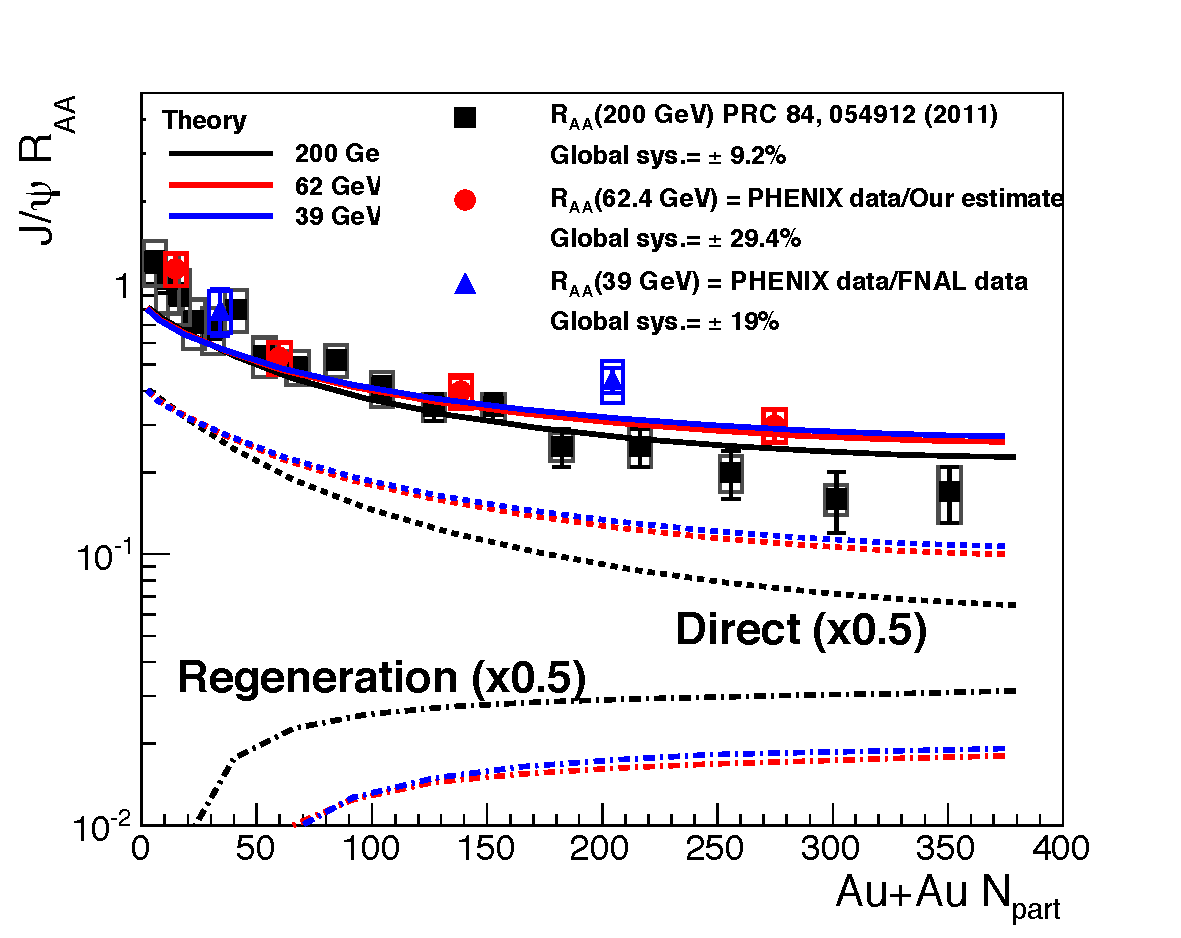
\includegraphics[width=0.8\textwidth]{fig/PHENIX_AuAu_excitation_function}
}
\caption[PHENIX data for \Jpsi\ production compared to theory calculations]{The nuclear modification factor for \Jpsi\ production for $\sqrt{s_{NN}}$=200, 62 and 39~GeV \AuAu\ collisions from
PHENIX~\cite{Adare:2012wf}, compared with theory calculations~\cite{Zhao:2010nk} showing the contributions from direct
suppression and regeneration.
}
\label{fig:PHENIX_excitation_function}
\end{figure}
%\begin{figure}[!ht]
%\centerline{
%\includegraphics[width=0.480\textwidth]{fig/ALICE_PHENIX_RAA_vs_dnchdeta}
%\includegraphics[width=0.48\textwidth, height=0.458\textwidth]{fig/PHENIX_ALICE_Jpsi_pT_comparison}
%}
%\caption{Left: Comparison of the nuclear modification factor for $J\psi$ production for $\sqrt{s_{NN}}=200$~GeV \AuAu\ collisions from
%PHENIX and for $\sqrt{s_{NN}}=2.76$~TeV \PbPb\ from ALICE. The data are plotted versus the charged
%particle multiplicity at midrapidity, which is used as a rough proxy for energy density. Right: The transverse momentum
%distributions for the same data sets, showing the low momentum enhancement that would be expected from a
%large coalescence contribution at the LHC energy.
%}
%\label{fig:ALICE_PHENIX_Jpsi_RAA}
%\end{figure}

\begin{figure}[!ht]
 \centering
 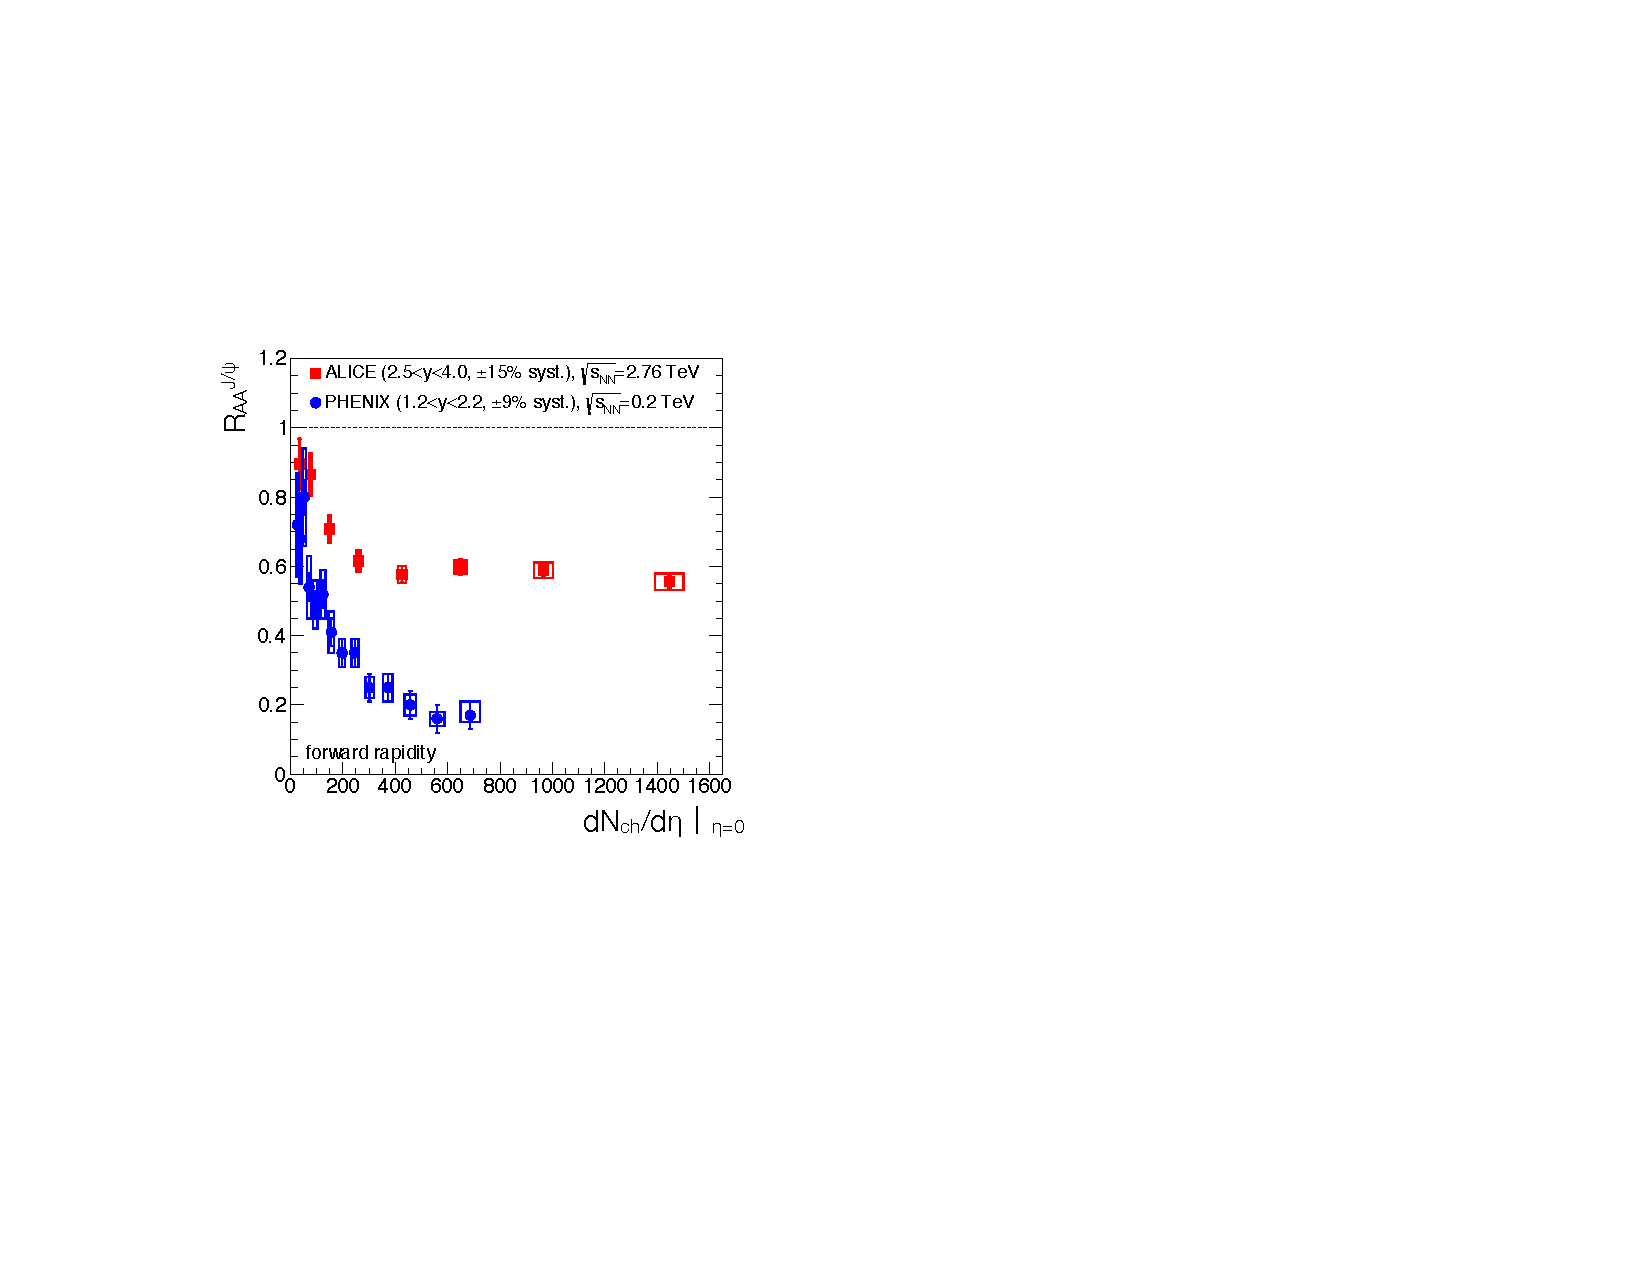
\includegraphics[width=0.435\linewidth]{fig/ALICE_PHENIX_Jpsi_cropped}
 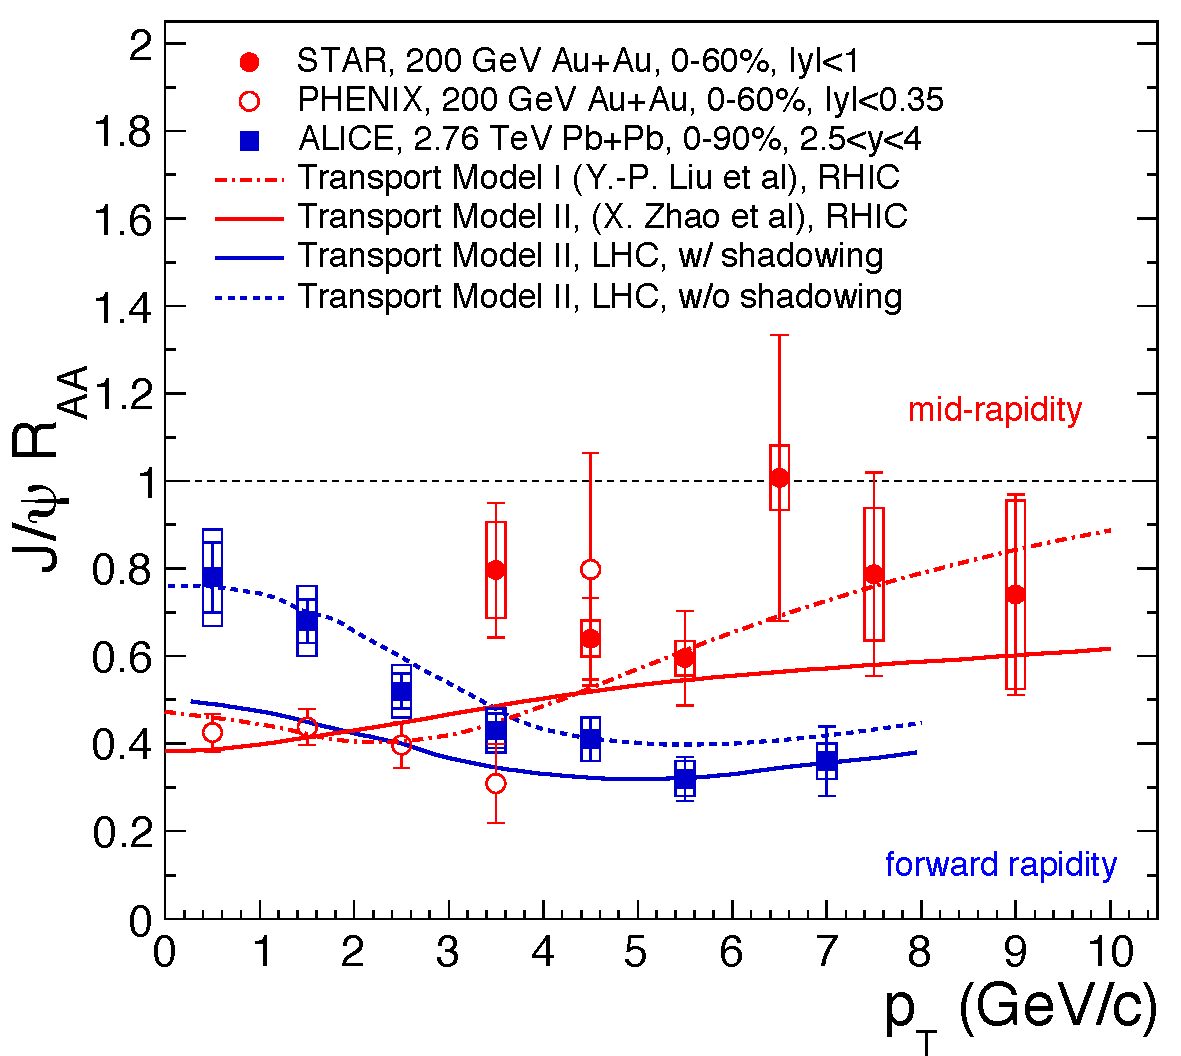
\includegraphics[width=0.46\linewidth]{fig/Jpsi_raa_vs_pt}
 \caption[Comparison of RHIC and LHC data on \Jpsi\ production]{
 Left: Comparison of the nuclear modification factor for \JPsi\ production for $\sqrt{s_{NN}}=200$~GeV \AuAu\ collisions from
PHENIX and for $\sqrt{s_{NN}}=2.76$~TeV \PbPb\ from ALICE~\cite{Andronic:2014zha}. The data are plotted versus the charged
particle multiplicity at midrapidity, which is used as a rough proxy for energy density. 
Right: The transverse momentum
distributions for the same data sets,
together with higher-momentum data from STAR\cite{Adamczyk:2012ey}
showing the low momentum enhancement that would be expected from a
large coalescence contribution at the LHC energy.
The data are compared to a transport model\cite{Liu:2009nb}
which incorporates the effects of gluon scattering and coalescence.
}
\label{fig:ALICE_PHENIX_Jpsi_RAA}
\end{figure}
	
	
The first \Jpsi\
data in Pb+Pb collisions at $\sqrt{s_{NN}}$ = 2.76 TeV from ALICE~\cite{Abelev:2012rv}, measured at forward
rapidity, are shown alongside forward rapidity PHENIX data in the left panel of Figure~\ref{fig:ALICE_PHENIX_Jpsi_RAA}. 
The suppression in central collisions is found to be far greater at RHIC than at the LHC. A similar result is found
at midrapidity. This is consistent with a predicted~\cite{Zhao:2011cv} strong coalescence component due to the 
large production rate of charm and anti-charm quarks in a central collision at the LHC. This explanation is 
corroborated by the transverse-momentum spectra~\cite{Adare:2006ns,Adamczyk:2012ey,Abelev:2013ila}, 
which exhibit the expected~\cite{Zhao:2011cv,Liu:2009nb}
low-momentum enhancement generated by the coalescence contribution, 
as shown in the right panel of 
Figure~\ref{fig:ALICE_PHENIX_Jpsi_RAA}.


\begin{figure}[!htb]
\centerline{
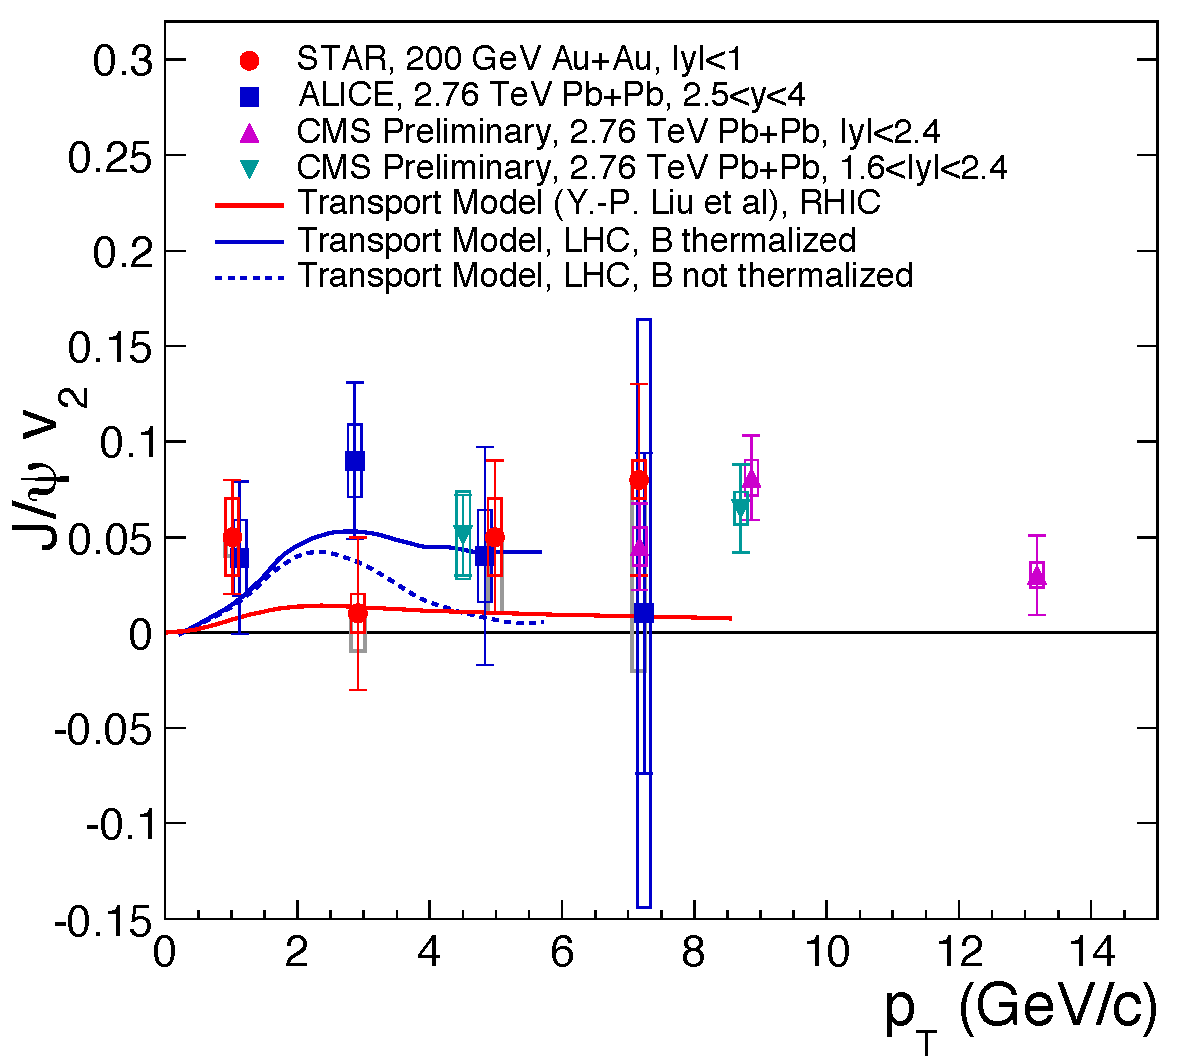
\includegraphics[width=0.8\textwidth]{fig/Jpsi_v2}
}
\caption[\Jpsi\ elliptic flow measurements at RHIC and LHC compared to theory]{
The transverse momentum dependent elliptic flow measurements of
\Jpsi\'s from STAR\cite{Adamczyk:2012pw}, ALICE\cite{ALICE:2013xna}, and CMS\cite{Moon:2014lia} compared with the theoretical calculations\cite{Liu:2009gx}.
}
\label{Fig:JPsi_v2}
\end{figure}

One of the crucial tests of the combined effects of color screening
and coalescence in \Jpsi\ production is provided by the measurement of the \Jpsi\ elliptic flow.
All other hadrons acquire flow velocities through their interaction with 
the QGP medium and simultaneously exhibit
significant elliptic flow and strong nuclear suppresssion. 
In contrast, disassociation of \Jpsi\'s from color screening
is predicted to result in strong nuclear modification with the absence of a flow signal, while
\Jpsi\'s later regenerated from coalescence production will carry flow from the thermalized charm quarks from which they are formed. 
Figure~\ref{Fig:JPsi_v2} 
shows the transverse momentum dependent elliptic flow measurements\cite{Adamczyk:2012pw,ALICE:2013xna,Moon:2014lia} 
from RHIC and the LHC together with a corresponding theoretical calculation\cite{Liu:2009gx}.
The data are consistent (within the current large statistical errors) with a model incorporating
disassociation from color screening at both RHIC and the LHC in combination with
significant regeneration of \Jpsi\'s at the LHC from coalescence of thermalized charm and anti-charm quarks,
The larger role of the coalescence  mechanism at the LHC results from the much 
higher cross section for charm production in the initial phase of the collision at LHC energies as compared to RHIC.
There is great promise that the  future availability of data sets 
with improved statistical precision
at the widely spaced collision energies of RHIC and the LHC, 
in combination with studies constraining CNM effects with \pA\ data, 
will lead to a quantitative
understanding of the role of coalescence from nearly thermalized charm and anti-charm quarks.
However, a more direct window on the Debye screening and dissociation effects alone is expected from
a systematic analysis of bottomonium production, as we will now discuss.
		
Bottomonium production is believed to have several advantages over charmonia as a probe of deconfinement in the
QGP. First, the $\Upsilon(1S)$, $\Upsilon(2S)$ and $\Upsilon(3S)$ states can all be observed with comparable
yields via their dilepton decays. Second, bottom production in central collisions is $\sim$ 0.05 pairs at RHIC
and $\sim$ 5 pairs at LHC~\cite{Brambilla:2010cs}. At RHIC, one expects this to effectively remove any contributions
from coalescence of bottom and anti-bottom quarks (although some care has to be taken, since the ratio of bottomonium over
open bottom states in pp collisions is $\sim$0.1\% and thus a factor of 10 smaller than in the charm
sector; thus, even small regeneration, even from a single pair in the reaction, can potentially be significant).
This makes the $\Upsilon$ suppression at RHIC dependent primarily on color screening and dissociation reactions,
as well as cold nuclear matter effects. Recent theoretical calculations~\cite{Emerick:2011xu} support the
assertion that the coalescence production for $\Upsilon$'s is small at RHIC. At LHC energies, 
bottom coalescence could become comparable with charm coalesence at RHIC, i.e. at the 10's of percent level.
Since the $\Upsilon(1S)$, $\Upsilon(2S)$ and $\Upsilon(3S)$ have a broad range of radii, precise measurements
of bottomonia modifications at RHIC and LHC energies will provide information over a large range of
binding energies at two widely different initial temperatures, for a case where the modification is dominated
by Debye screening effects.
	
The CMS experiment at the LHC has mass resolution that is sufficient to cleanly separate all three of the
$\Upsilon$ states at midrapidity using dimuon decays~\cite{Chatrchyan:2012lxa}. The data obtained in Pb+Pb collisions at
$\sqrt{s_{NN}}$=2.76 TeV for the $\Upsilon(1S)$ and $\Upsilon(2S)$ states are shown in
Figure~\ref{fig:CMS_Upsilons}, where they are compared with a model calculation~\cite{Emerick:2011xu} that includes
both cold nuclear matter effects and regeneration. The data show much stronger suppression of the $\Upsilon(2S)$
than the $\Upsilon(1S)$. The $\Upsilon(3S)$ is even more strongly suppressed, 
and as a result the yield is too small to determine accurately the nuclear suppression factor. 
The theory is in good agreement with the data, although better statistical precision is needed for strong
theoretical constraints. Future Pb+Pb data at the LHC will be measured at $\sqrt{s_{NN}}$=5.5 TeV, and will have greatly increased
statistical precision.
	
	
\begin{figure}[!htb]
\centerline{
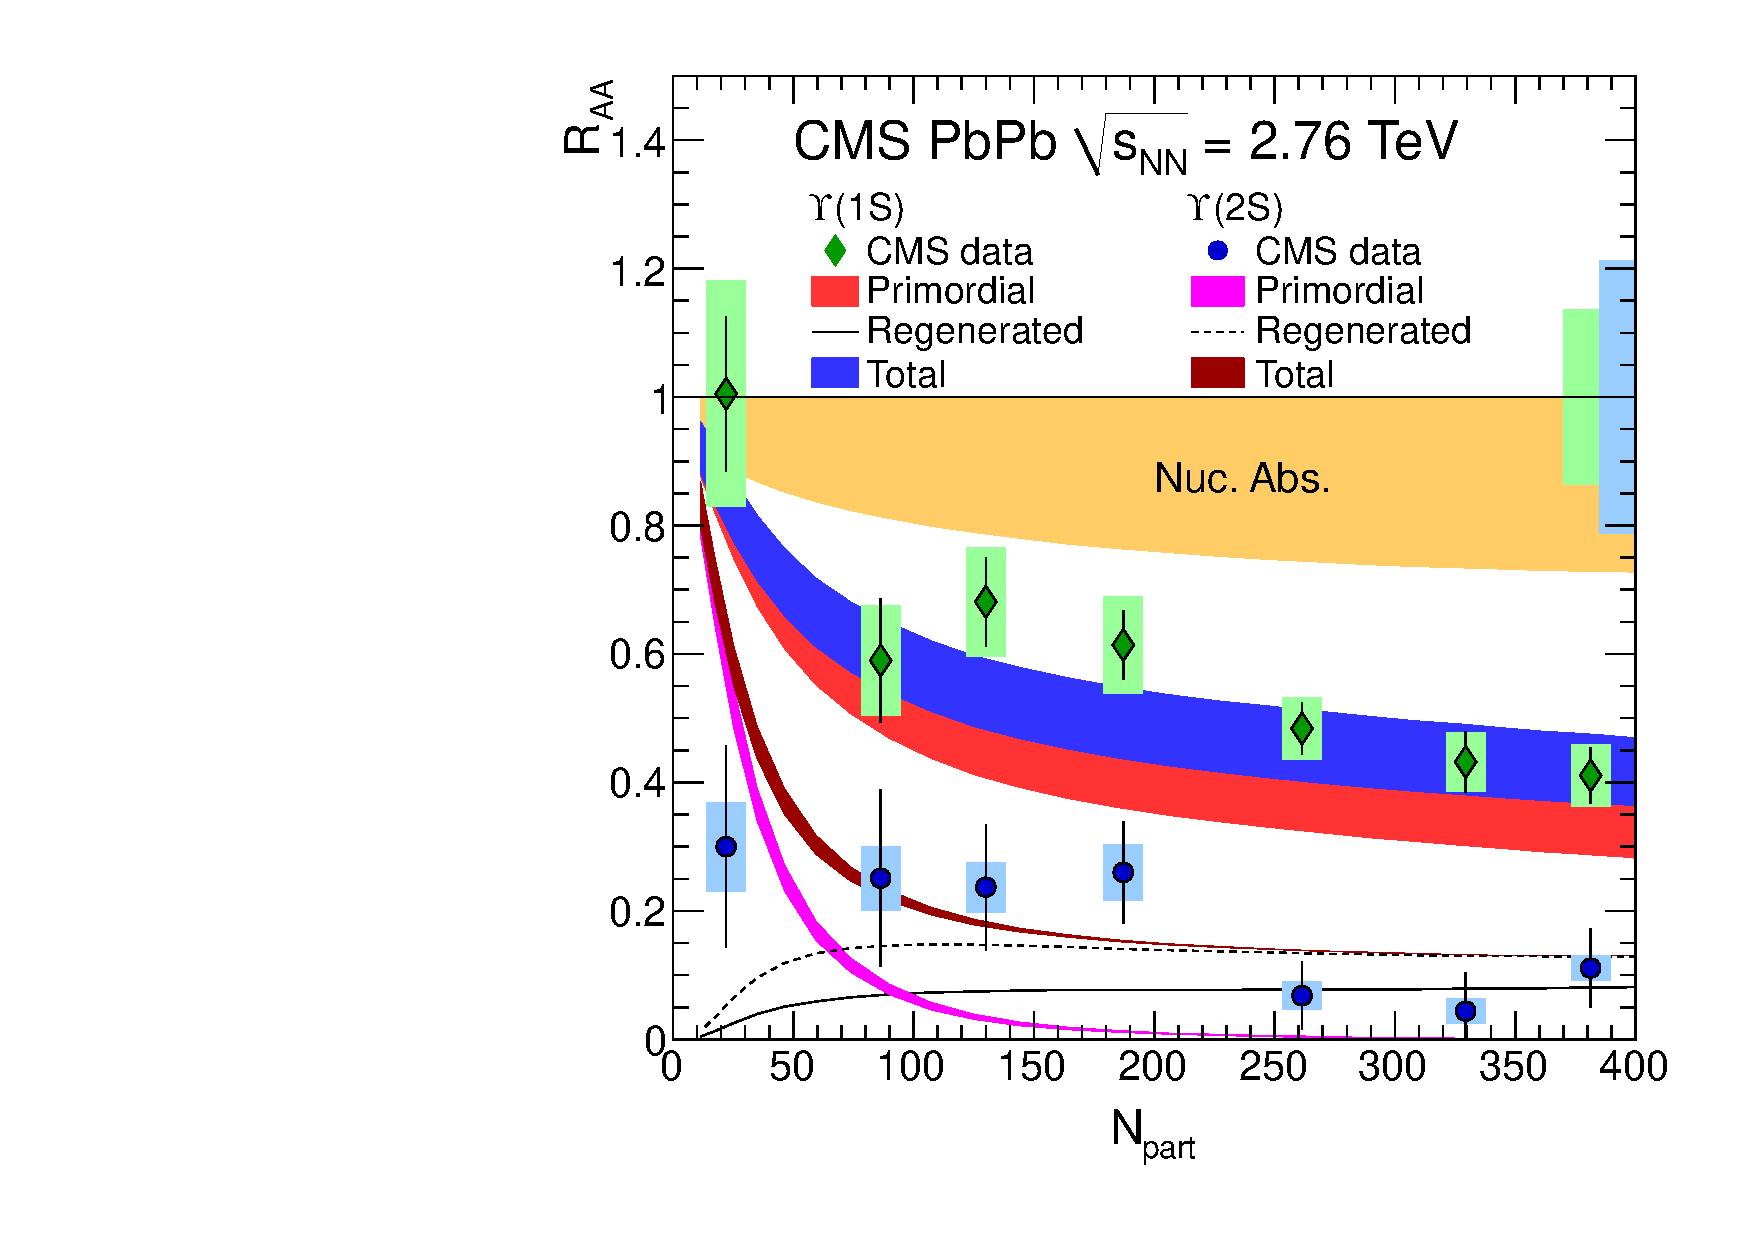
\includegraphics[width=0.7\textwidth]{fig/CMS_Upsilon_RAA_Rapp_theory}
}
\caption[CMS measurements of $\Upsilon$ production compared to theory]{The nuclear suppression factor $R_{AA}$ for the $\Upsilon(1S)$ and $\Upsilon(2S)$ states measured at $\sqrt{s_{NN}}$=2.76 TeV
by CMS~\cite{Chatrchyan:2012lxa}. The theory calculation~\cite{Emerick:2011xu} includes cold nuclear matter effects
and the contributions from the surviving primordial \Jpsi\ and those which are formed by regeneration are shown, as well
as the total.
}
\label{fig:CMS_Upsilons}
\end{figure}
	
	
By the end of Run 3 at
the LHC (approximately 2023) CMS will have measured very precise cross sections for the three
$\Upsilon$ states in p+p, p+Pb and Pb+Pb collisions. A mass-resolved measurement of the modifications
of the three upsilon states with similar precision at RHIC energy would be extremely valuable for all of
the reasons outlined above. However $\Upsilon$ measurements at RHIC have been hampered by a
combination of low cross sections and acceptance, and insufficient momentum resolution to resolve the
three states. At RHIC there are measurements of the modification of the three states
combined in Au+Au by PHENIX~\cite{Adare:2014hje} and STAR~\cite{Adamczyk:2013poh}. These data
are shown in Figure~\ref{fig:RHIC_Upsilons}, along with two theory
calculations\cite{Emerick:2011xu,Strickland:2011aa} of the modification of the three Upsilon states combined.
The data available so far have limited statistical precision, and do not place strong constraints on models.
	
\begin{figure}[!htb]
\centerline{
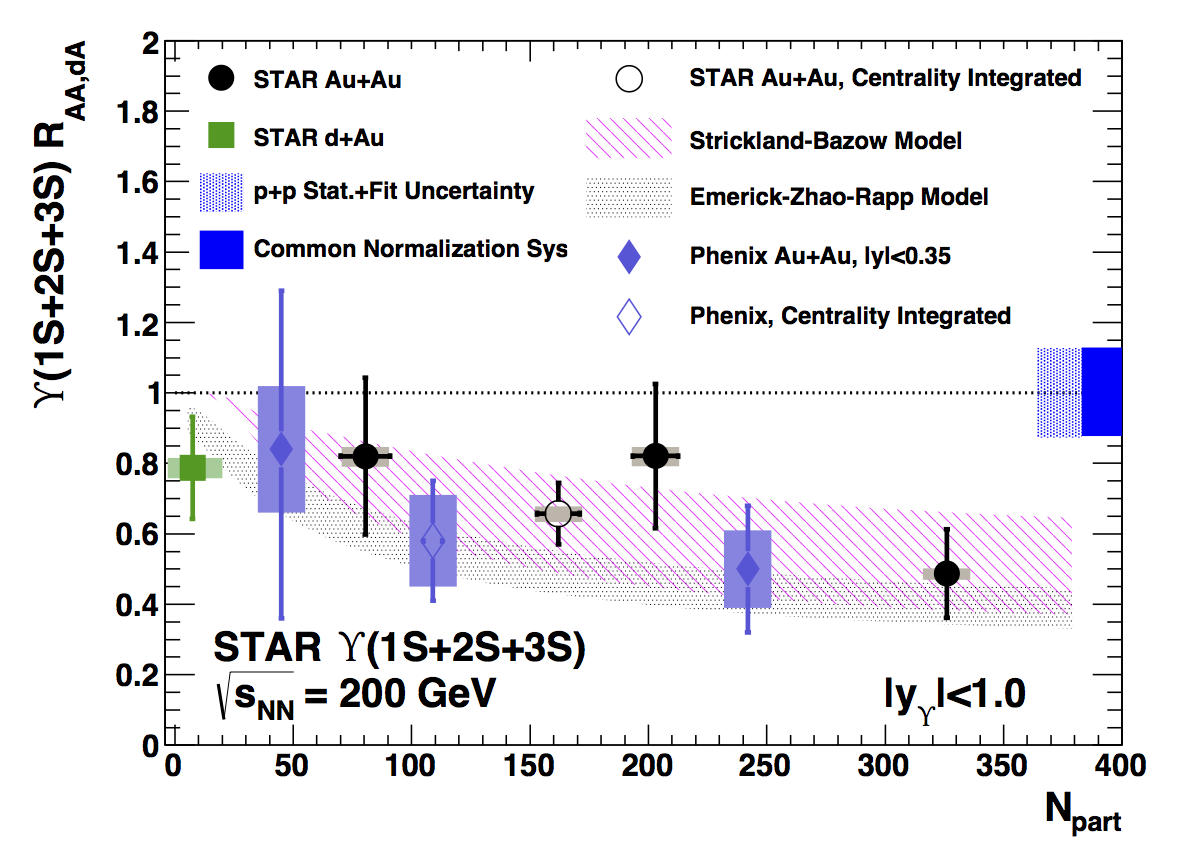
\includegraphics[width=0.9\textwidth]{fig/RHIC_Upsilons}
}
\caption[RHIC measurements of $\Upsilon$ production compared to theory]{The nuclear suppression factor $R_{AA}$ for the $\Upsilon(1S+2S+3S)$ states measured at $\sqrt{s_{NN}}$=200 GeV
by PHENIX\cite{Adare:2014hje} and STAR~\cite{Adamczyk:2013poh}. The theory calculations are from~\cite{Emerick:2011xu,Strickland:2011aa},
}
\label{fig:RHIC_Upsilons}
\end{figure}
	
There are, however, good prospects for future $\Upsilon$ measurements at RHIC. STAR recorded data in the 2014
RHIC run with the new Muon Telescope Detector (MTD), which measures dimuons at midrapidity~\cite{Ruan:2009ug}.
The MTD has coverage of $|\eta| < 0.5$, with about 45\% effective azimuthal coverage. It will have a
muon to pion enhancement factor of $\sim$ 50, and the mass resolution will provide a clean separation
of the $\Upsilon(1S)$ from the $\Upsilon(2S+3S)$, and likely the ability to separate the 2S and 3S states by fitting.
	
On a longer time scale, the proposed sPHENIX detector~\cite{Aidala:2012nz} at RHIC 
discussed in Section~\ref{Sec:FacilitiesFuture} would begin operation in
2021. It is designed to measure $\Upsilon$'s via their dielectron decays at midrapidity. The 100 MeV mass
resolution is sufficient to cleanly separate all three $\Upsilon$ states. Pions are suppressed relative to electrons
by a factor of 90. A combination of very high luminosity, good mass resolution, good background rejection and large
acceptance (about a factor of 7 larger than the MTD) leads to a data set with precision comparable to that expected
from the CMS data by 2023, and on a similar time scale.